\documentclass[10pt]{beamer}
\mode<presentation>
{
\usetheme{CambridgeUS}
\usecolortheme{dolphin}
}
\usepackage{etex}
\usepackage[english]{babel}
\usepackage{amstext,amsthm,amsmath,amsfonts,latexsym,graphicx,amssymb,epsfig,epsf,psfrag}
\usepackage{pgfpages,xcolor,subfigure,pstricks}
\usepackage{fancyhdr}
\usepackage{pst-all}
\graphicspath{ {figures/} }

%\hypersetup{pdfpagemode=FullScreen}
\usefonttheme{professionalfonts}
\setbeamertemplate{footline}[frame number]
%\setbeamertemplate{footline}{\hfill\insertframenumber~\vrule~\inserttotalframenumber}
\setbeamertemplate{theorem}[ams style]
\setbeamertemplate{theorems}[numbered]
\definecolor{purple}{RGB}{255,0,204}

\newcommand{\defeq}{\triangleq}
\newcommand{\Pp}{\mathbb{P}}
\newcommand{\E}{\mathbb{E}}
\newcommand{\N}{\mathbb{N}}
\newcommand{\Z}{\mathbb{Z}}
\newcommand{\Zp}{\mathbb{Z}_{+}}
\newcommand{\R}{\mathbb{R}}
\newcommand{\Rp}{\R_{+}}
\newcommand{\C}{\mathbb{C}}
\newcommand{\Q}{\mathbb{Q}}
\newcommand{\F}{\mathbb{F}}
\newcommand{\Zw}{\mathbb{Z}[\omega]}
\newcommand{\Zi}{\mathbb{Z}[i]}
\newcommand{\mc}{\mathcal}
\newcommand{\mbb}{\mathbb}

\usecolortheme[RGB={0,100,0}]{structure}
\setbeamertemplate{itemize item}[circle]
\setbeamertemplate{itemize subitem}[rectangle]
\setbeamertemplate{itemize subsubitem}{$-$}
\setbeamertemplate{blocks}[rounded][shadow=true]
\setbeamertemplate{navigation symbols}{} % get rid of navigation symbols
%\logo{\includegraphics[height=1cm,keepaspectratio]{greentouch.eps}}

%\AtBeginSubsection[]
%{
%  \begin{frame}<beamer>{Outline}
%    \tableofcontents[currentsection,currentsubsection]
%  \end{frame}
%}

\begin{document}
\title{\bf Multilevel Lattices based on Spatially Coupled LDPC codes with Applications}
\author{{\bf Avinash Vem,  \bf Yu-Chih Huang,  \bf Krishna R. Narayanan, \\ \& Henry D. Pfister} \\ \vspace{2pt} \textit{Texas A\&M University}}

\date{ISIT '14} % if no date wanted, keep it blank
\frame{\titlepage}

\begin{frame}
	\frametitle{Outline}
	\tableofcontents
\end{frame}

\section{Introduction}
\subsection{Motivation}
\begin{frame}\frametitle{Lattices and Lattice Codes}


    		\begin{itemize}
    		 \item Efficient structures for packing, covering, channel coding \& quantization
            \item Single user Gaussian channel - Erez and Zamir
			\item Coding with side information - Wyner-Ziv and Costa, Zamir, Erez and Shamai
			\item Secrecy - He and Yener
			\item Dirty multiple access channel - Philosof, Khisti, Erez and Zamir
	\end{itemize}
	
``Lattices are everywhere" by Ram Zamir
\end{frame}

\begin{frame}

New perspectives for dealing with interference:
      \begin{itemize}
     		\item<1-> Interference alignment - Sridharan, Jafarian, Vishwanath and Jafar
			\item<2-> Compute-and-forward - Nazer \& Gastpar
			\item<2-> Physical layer network coding - Wilson et al, Nam et al
      \end{itemize}
			\vspace{2.5em}
			
	\begin{figure}
		\centering
		\only<1->{\includegraphics[width=4in]{IC_model_ISIT}}
	\end{figure}
\end{frame}  

\begin{frame}\frametitle{Lattices and Lattice Codes}
\begin{block}{}
			\begin{itemize}
				\item Above schemes are all based on good lattice codes.
				\item	\textit{Poltyrev-}good lattices are at the core of such lattice coding schemes
			\end{itemize}
\end{block}
\pause
\vspace{0.3in}
		\begin{block}{Motivating questions}
			\begin{center}
				\begin{itemize}
						\item These results are all based on Construction-A.
						\item<2-> Is this construction fundamental to good lattices?
						\item<2-> Can we work with just binary codes under practical decoding schemes?
				\end{itemize}
			\end{center}
		\end{block}

\end{frame}


\begin{frame}\frametitle{Main Results in this Talk}

			\begin{block}{Codes over $\mathbb{F}_{2}$ and BP decoding suffice}
				\vspace{1em}
	\begin{itemize}
			\item Recall Forney et al's result - based on nested random binary linear codes
			\item Propose capacity-achieving nested SC LDPC ensemble
			\item Construct lattices using Construction-D, based on the above ensemble
			\item Show existence of sequence of lattices that are \textit{Poltyrev}-good under BP 
	\end{itemize}			
			\end{block}
\pause
\vspace{2em}
		\begin{block}{Applications}
			    \begin{itemize}
        \item As an application, propose {\blue Symmetric Interference Channel}
        \item Can be applied to other problems which adopt Construction A lattices
    			\end{itemize}
		\end{block}

\end{frame}


\subsection{Construction D}
\begin{frame}\frametitle{Construction D with $L$ levels}
\begin{itemize}
    \item Barnes and Sloane '83, Forney, Chung and Trott '00, Yan, Ling, Wu ' 13
				 \vspace{0.5em}
	 \item Choose  $G_{1}\subseteq \ldots \subseteq G_{L}$ where $G_{l}$ is a gen matrix of code $\mc{C}_{l}$ over $\mathbb{F}_{2}$.
				 \vspace{.5em}
	\item<2->  $  \underline{\lambda} = \underline{w}_1 \mathbf{G}_1 + 2 \underline{w}_2 \mathbf{G}_2 \ldots +2^{L-1} \underline{w}_{L-1} \mathbf{G}_{L-1} +2^{L}\mathbb{Z}^{N} \in \Lambda$
\end{itemize}
				\vspace{0.2in}
    \begin{columns}[t]      
 	      \begin{column}{0.6\textwidth}
            \begin{figure}
			\only<2>	{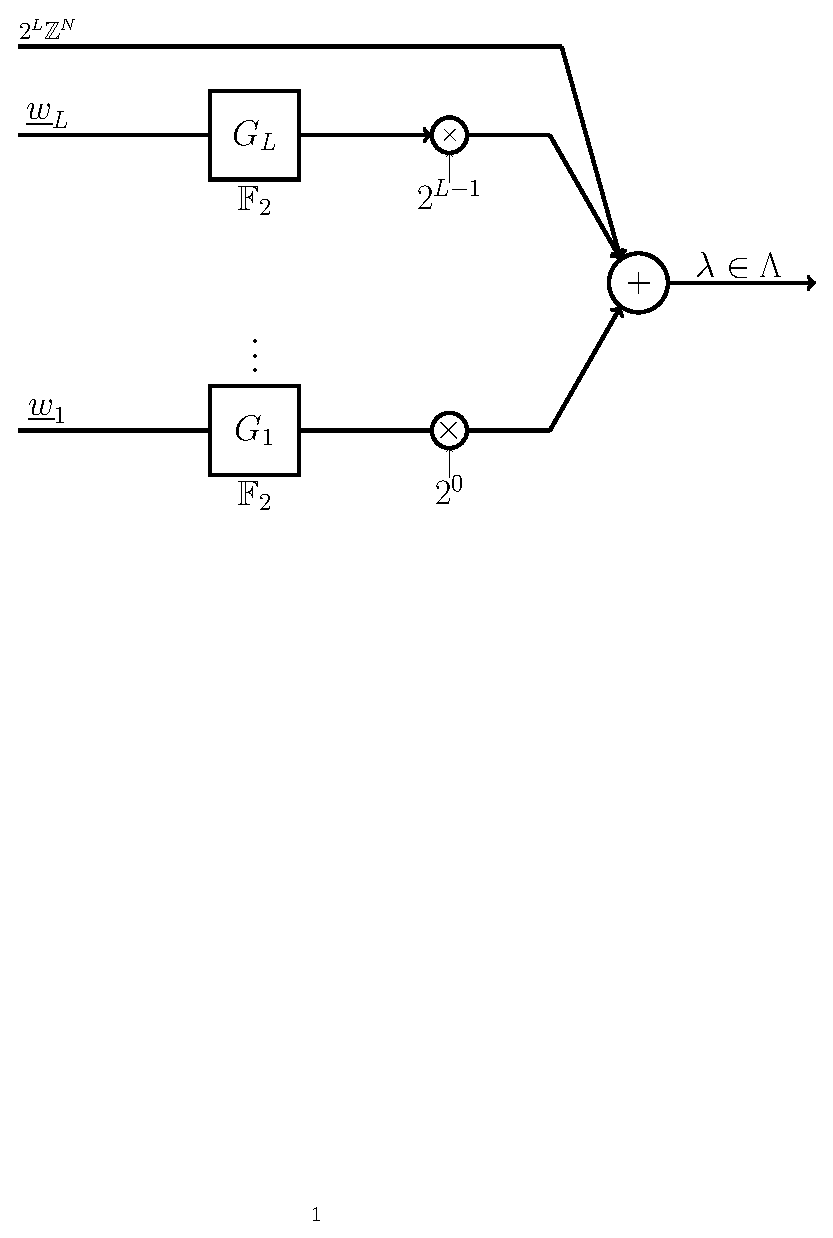
\includegraphics[width=2.5in]{lattice_Constr_D1}}
            \end{figure}
        \end{column}

		\begin{column}{0.39\textwidth}
						\begin{figure}
						\only<1->	{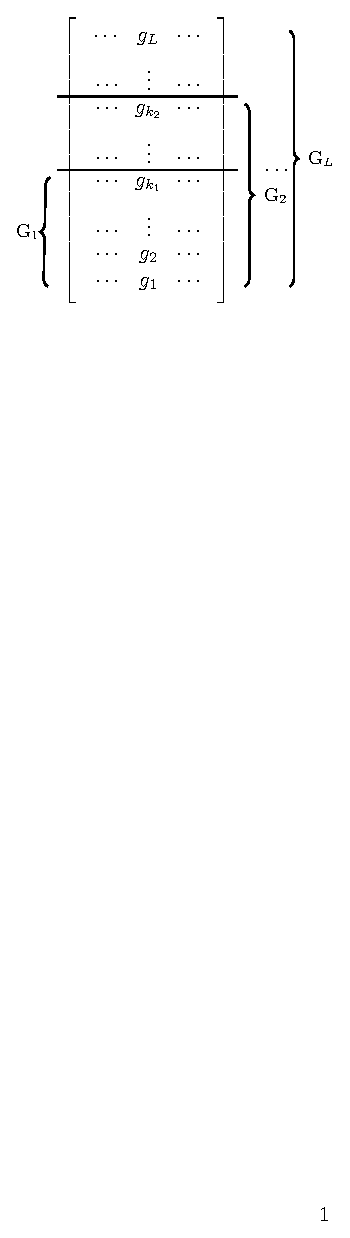
\includegraphics[width=0.95\columnwidth]{Nested_generator_matrix}} % both of these ways work
				  	\end{figure}
        \end{column}
    \end{columns}    
\end{frame}


\begin{frame}\frametitle{Multi-Level Decoding(Successive Decoding) }
      \begin{itemize}
        \item $\underline{y} = \boxed{\underline{w}_1 \mathbf{G}_1 + 2 \underline{w}_2 \mathbf{G}_2 \ldots +2^{L-1} \underline{w}_{L-1} \mathbf{G}_{L-1} +2^{L}\mathbb{Z}^{N}} + \underline{n}$
         \vspace{0.05in}	
         \item $\underline{y}$ mod 2 = $ \left[\,\underline{w}_1 \mathbf{G}_1 + \underline{n}\,\right] $ mod 2 = $\underline{w}_1 \odot \mathbf{G}            _1 + \boxed{\underline{n} \mod 2}$
         \vspace{0.05in}
		\item Decode $\underline{w}_1$, reconstruct $\underline{w}_1 \mathbf{G}_1$ and subtract from $\underline{y}$
         \vspace{0.2in}
    \end{itemize}
            \begin{figure}
					\includegraphics[width=3in]{multi_stage_decode}
            \end{figure}
	\end{frame}


\begin{frame}
%        \begin{theorem}[Forney, Trott \& Chung]
%            For an AWGN channel with noise variance $\sigma^{2}$ per dimension, there exists a Construction D lattice based on binary linear codes $\mc{C}_{1}\subseteq \mc{C}_{2}\ldots \subseteq \mc{C}_{r}$ such that the Volume-to-Noise(VNR) ratio is arbitrarily close to $1$ and the probability of error is arbitrarily small.
%       \end{theorem}
        \begin{theorem}[Forney, Trott \& Chung]
There exists a sequence of Construction D lattices based on $\mc{C}_{1}\subseteq \mc{C}_{2}\ldots \subseteq \mc{C}_{L}$ such that the VNR $\rightarrow 1$ and the $Pr(\lambda,\sigma^{2})\rightarrow 0$.
       \end{theorem}

\begin{itemize}
\item Take $L$ large enough.
\item It's sufficient that $\mc{C}_{i}$ at each level is capacity achieving for the mod-2 AWGN channel.
\end{itemize}
\pause
\vspace{0.4in}
Objective:
\begin{itemize}
\item Capacity achieving nested code constructions, preferably under BP decoding.
\end{itemize}
\end{frame}

\section{Proposed Lattices}
\subsection{Construction}
\begin{frame}\frametitle{Proposed Nested Spatially-Coupled LDPC Ensemble}
    \begin{enumerate}
        \item<1-> Begin with a $(d_v^1,d_c)$ SC LDPC code. For ex, $(d_v^1=3,d_c=6,L=3,w=2)$. 
        \item<1-> Group check nodes into type $\mathcal{T}_k$, $k\in\{1,\ldots,d_v^1\}$
         \vspace{2pt}
        \item<2-> Remove all check nodes of type $\mathcal{T}_1,\ldots,\mathcal{T}_{d_v^1-d_v^2}$. Ex: $(d_{v}^{2}=2,6)$ sup-code.
                 \vspace{2pt}
        \item<3-> Results in a super-code that is a $(d_v^2,d_c)$ SC LDPC code.
    \end{enumerate}
    \vspace{0.15in}
    \begin{figure}
        \begin{center}
 	        \only<1>{\includegraphics[width=3.2in]{Basegraph_ISIT1}}
         \only<2>{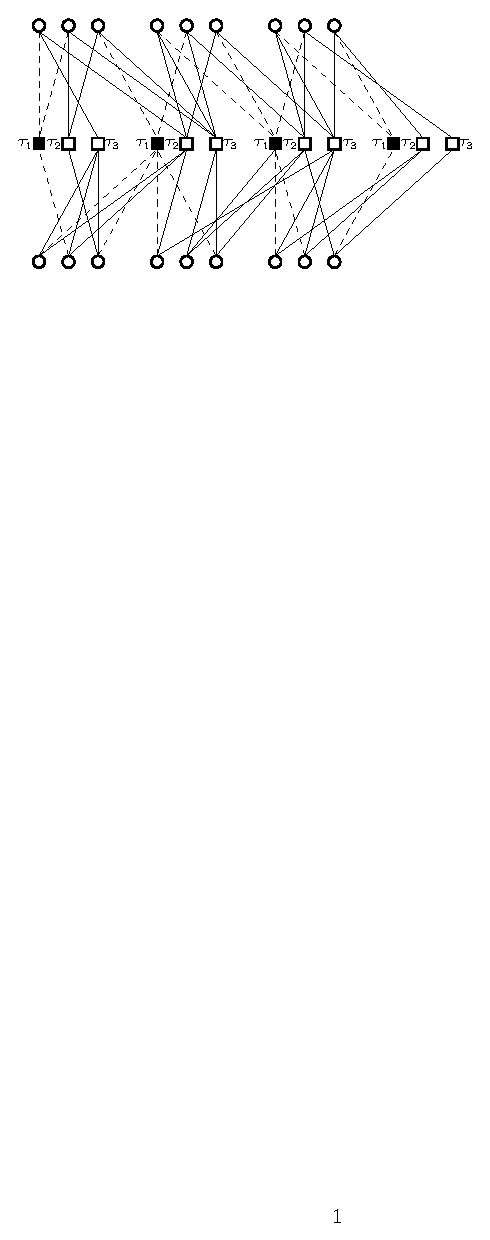
\includegraphics[width=3.2in]{Basegraph_ISIT2}}
         \only<3>{\includegraphics[width=3.1in]{Basegraph_ISIT3}}
        \end{center}
    \end{figure}
\end{frame}
         
\begin{frame}\frametitle{Lattice Design based on the proposed Nested SC LDPC ensemble}
\begin{enumerate}
\item For a given $\sigma$, compute the capacity of the mod-2 AWGN channel at each level:
		$$
         \underline{y_{i}}= \underline{w}_i \mathbf{G}_i +\frac{1}{2^{i-1}} \underline{n}\mod 2=\underline{w}_i \odot \mathbf{G}_i + \boxed{\frac{1}{2^{i-1}}\underline{n} \mod 2}
         $$
         \vspace{0.08in}

\item Fix check node degree $d_{c}$. Choose $d_{v}^{1},\ldots ,d_{v}^{r}$ such that the rate of the code at each level is arbitrarily close to the capacity at the respective level.
\end{enumerate}
\pause
\begin{lemma}\label{lemma:nested_G}
    Given nested binary linear codes $\mc{C}_{1}\subseteq \mc{C}_{2}\subseteq\ldots \subseteq\mc{C}_{r}$ there exists nested generator matrices for these codes.
\end{lemma}
\end{frame}

\subsection{Poltyrev Goodness}
\begin{frame}\frametitle{Proposed Ensemble is Capacity achieving}
\begin{theorem}
Each code ensemble in the proposed nested Spatially-Coupled LDPC ensemble is capacity achieving. 
\end{theorem}    
\begin{proof}
\begin{itemize}
        \item Show that the mod 2 AWGN channel is BMS.
        \item Each derived protograph has the same spatially coupled structure.
        \item The proof follows from Kudekar \& Urbanke, Kumar \& Pfister's  results.
    \end{itemize}
\end{proof}
\end{frame}

\begin{frame}\frametitle{Proposed Lattices are Poltyrev-Good}
\begin{theorem}
There exists a sequence of SC LDPC lattices with VNR$(\Lambda,\sigma^{2})\rightarrow 1$ for which, under multistage BP decoding, $\mbb{E}\left[P(\lambda,\sigma^{2})\right]\rightarrow 0$ as $w,L,M  \rightarrow \infty$.
\end{theorem}    
\begin{proof}
%Follows from Forney's result and the fact that the proposed nested ensemble achieve capacity.
\begin{itemize}
\item The proposed nested ensemble achieve capacity.
\item Follows from Forney's result.
\end{itemize}

\end{proof}
\vspace{0.3in}
\pause
\begin{itemize}
        \item Binary codes and more importantly practical BP decoding suffices. 
        \item Practically we observe that two levels of coding gets you lattices very close to Poltyrev limit.
    \end{itemize}
\end{frame}
	
\begin{frame}\frametitle{Design Example of Poltyrev-Good Lattice}
A target block error probability of $10^{-4}$ in the uncoded level gives $\sigma_{L}=0.08$
\begin{enumerate}
\item  Capacities for the mod 2 AWGN  channel for respective levels: 
\vspace{0.1in}
\begin{center}
\begin{tabular}{| c | c | c | c | }
\hline
 & Level L-1   &  Level L-2  & Level L-3 \\
\hline 
$\sigma_{\text{eff}}$ & 0.16   &  0.32  & 0.64 \\ \hline
 Cap                             &  0.99 & 0.57 & 0.02 \\   \hline
 (14,30) (3,30)         &  0.9 & 0.533 & 0 \\   \hline
\end{tabular}
\end{center}
\pause
\vspace{0.1in}
\item Fix L=3 and use $(3,30)$, $(14,30)$ nested SC LDPC codes.
%\item With the SC parameters $(L,w)=(32,4)$, $\sigma_{\text{DE}}= 0.3184$ whereas $\sigma_{\text{DE}}= 0.3143$.
\vspace{0.07in}
\begin{center}
\begin{tabular}{c c c c c c c}
\hline  \hline
$(d_{c},d_{v}^{1},d_{v}^{2})$ &(L,w)& $P(\Z_{4},\sigma^{2})$ & $\sigma_{\text{max}}$ &$\text{VNR}$ &$\text{VNR}_{\text{rate-loss}}$\\
\hline
(30,14,3) & (32,4) & $5 \times 10^{-10}$ & 0.3184 & 1.02dB & 1.347dB\pause \\
(60, 26, 3)& (72, 12)& $5 \times 10^{-10}$ & 0.3200 &0.482dB & 0.927dB\\
(60, 27, 3)& (64, 9)& $5 \times 10^{-10}$  &  0.3203 & 0.57dB & 0.951dB\\
%(60, 42, 3)& (80, 16)& $1 \times 10^{-6}$ & 0.4020 & 0.106dB &0.952dB\\
\end{tabular}
\end{center}
\end{enumerate}
\end{frame}

\begin{frame}\frametitle{Alternate Nested SC LDPC ensemble}
\begin{itemize}
		\item<1-> Derive a lower rate code by ``splitting the checks"
					\vspace{2pt}
		\item<1-> Consider a $(3,8)$ code
					\vspace{2pt}
		\item<2-> Split each check into ``two" checks to derive a $(3,4)$ sub-code
					\vspace{2pt}
		\item<2-> Easy to prove that resulting code is from the $(3,4)$ SC LDPC ensemble
\end{itemize}
\vspace{0.3in}
    \begin{figure}
        \begin{center}
         \only<1>{\includegraphics[width=2in]{Constr1_graph1}}
           \only<2>{\includegraphics[width=2in]{Constr1_graph2}}
        \end{center}
    \end{figure}
\end{frame}

\begin{frame}\frametitle{Simulation Results}

\begin{figure}
\begin{center}
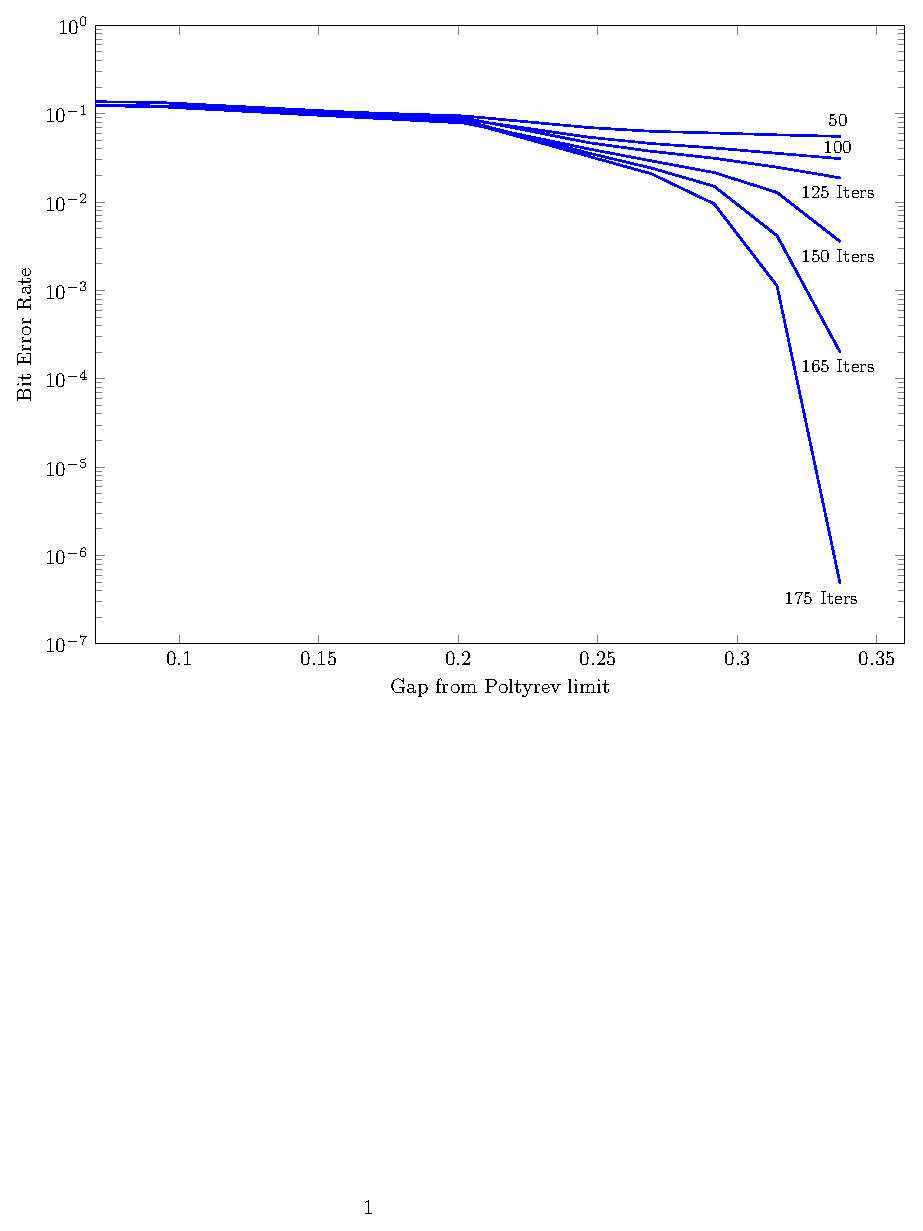
\includegraphics[width=3.2in]{BER_iters_4_72_9}
\end{center}
\end{figure}
\only<2->{  Note that the Block Error Probability is $10^{-4}$ at uncoded level.}
\end{frame}

\section{Application}
\subsection{Symmetric Interference Channel}
\begin{frame}\frametitle{3-User Symmetric Interference Channel}
	\begin{figure}
	\centering
    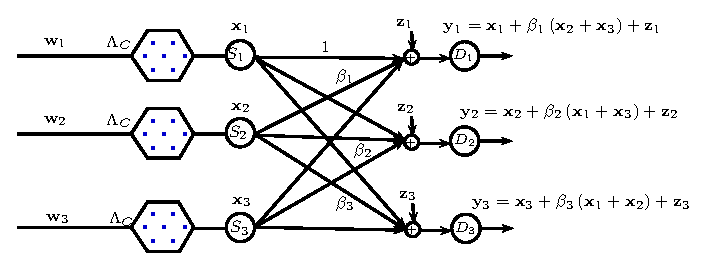
\includegraphics[width=4in]{IC_model_ISIT_3user}
	\end{figure}
\pause
\begin{itemize}
\item $\mathbf{x}_{i}\in \Lambda_{C}\defeq \Lambda \cap \mathbb{Z}_{4}^{N}$ is transmitted.
\vspace{0.2in}
\end{itemize}
\end{frame}


\begin{frame}\frametitle{Symmetric Interference Channel - Decoding Sums }


 Interference at Destination 1:
\begin{align*}
 \mathbf{x}_{2}+\mathbf{x}_{3}&= (\underline{w}_2^1+\underline{w}_3^1) \mathbf{G}_1 + 2 (\underline{w}_2^2+\underline{w}_3^2) \mathbf{G}_2 + 4\mathbf{k}_{23}\\
& = (\underline{w}_2^1 \oplus \underline{w}_3^1) \mathbf{G}_1 + 2 (\underline{c}_{23}^{1} \oplus \underline{w}_2^2 \oplus \underline{w}_3^2) \mathbf{G}_2 + 4(\underline{c}_{23}^{2} +\mathbf{k}_{23})\mathbf{Z}_{}
\end{align*}

where the carry overs are

\begin{align*}
& \underline{c}_{23}^{1}=0.5\left(\underline{w}_{1}^{1}+\underline{w}_{1}^{2}-\underline{w}_{1}^{1}\oplus\underline{w}_{1}^{2}\right), \\
& \underline{c}_{23}^{2}=0.5\left(\underline{c}_{23}^{1}+\underline{w}_{2}^{1}+\underline{w}_{2}^{2}-\underline{c}_{23}^{1}\oplus\underline{w}_{2}^{1} \oplus \underline{w}_{2}^{2}\right)
\end{align*}
%are carryovers from first and second levels respectively.
%and $\mathbf{k}_{23}=\mathbf{k}_{2}+\mathbf{k}_{3}+\sum_{1}^{k_{2}}c_{2i}\mathbf{g}_{i}\in\Z^{n}$. 
\begin{columns}
        \begin{column}{0.47\textwidth}
            \begin{figure}
               \includegraphics[width=2in]{lattice_Constr_D1_user1}
            \end{figure}
        \end{column}
        \begin{column}{0.47\textwidth}
            \begin{figure}
                \includegraphics[width=2in]{lattice_Constr_D1_user2}
            \end{figure}
        \end{column}
\end{columns}
\end{frame}

%\begin{frame}\frametitle{Simulations - Gap from Strong Interference regime}
%
%\end{frame}


%\begin{frame}\frametitle{Symmetric Interference Channel(SIC)}
%\begin{itemize}
%\item For each user $i$, $X_{i}\in \Lambda_{C}\defeq \Lambda \cap \mathbb{Z}_{4}^{N}$ is transmitted.
% \vspace{5pt}
%\item At receiver 1 :
%\[
%Y_{1}=X_{1}+\beta \left( X_{2}+X_{3} \right)+ N
%\]
%where $N \sim \mathcal{N}(0,\sigma^{2}\cdot I)$.
%\end{itemize}
%    \vspace{20pt}
%    \begin{figure}
%     \begin{center}
%       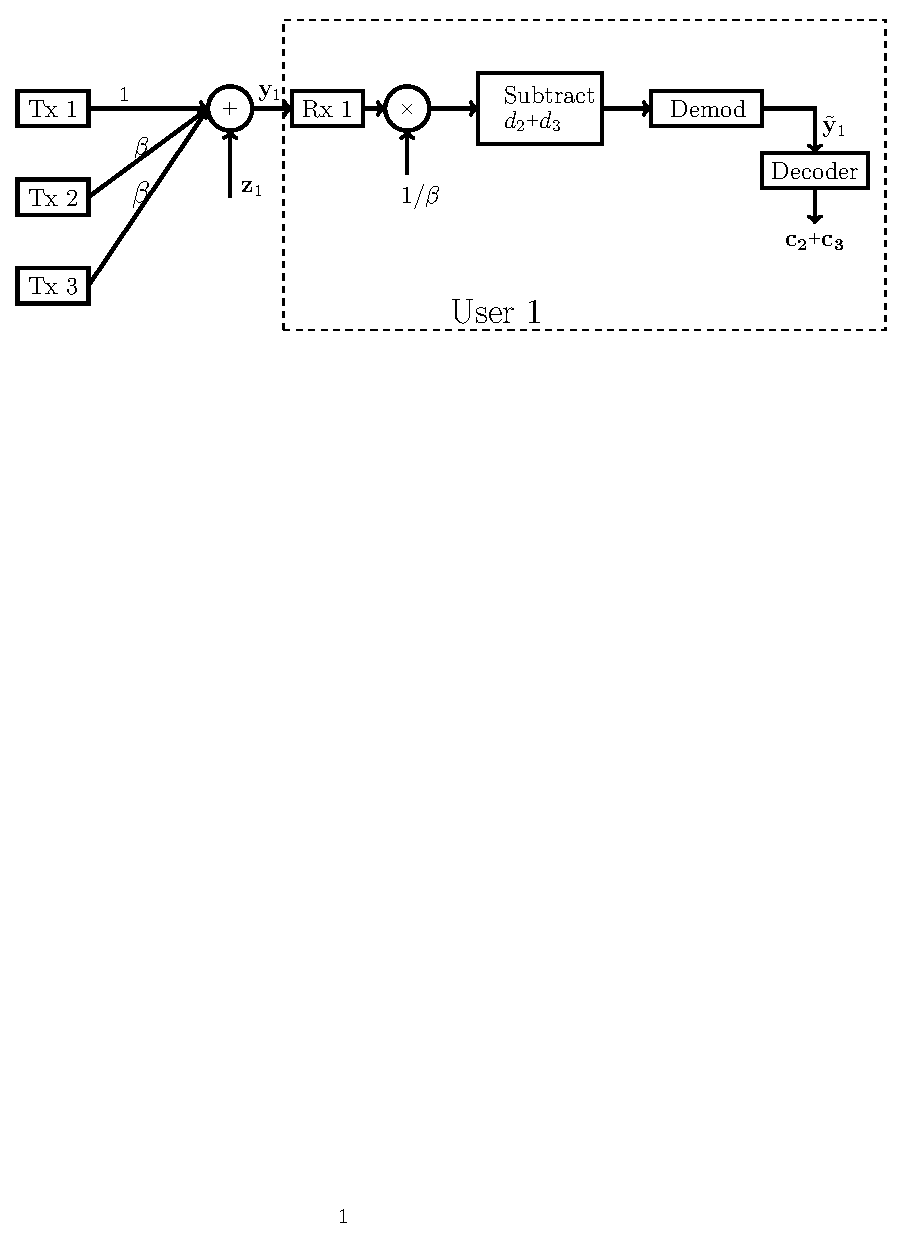
\includegraphics[width=3.5in]{SIC_decoder}
%      \end{center}
%    \end{figure}
%\end{frame}


\begin{frame}\frametitle{Achievable Information Rates}
    \begin{figure}
        \begin{center}
            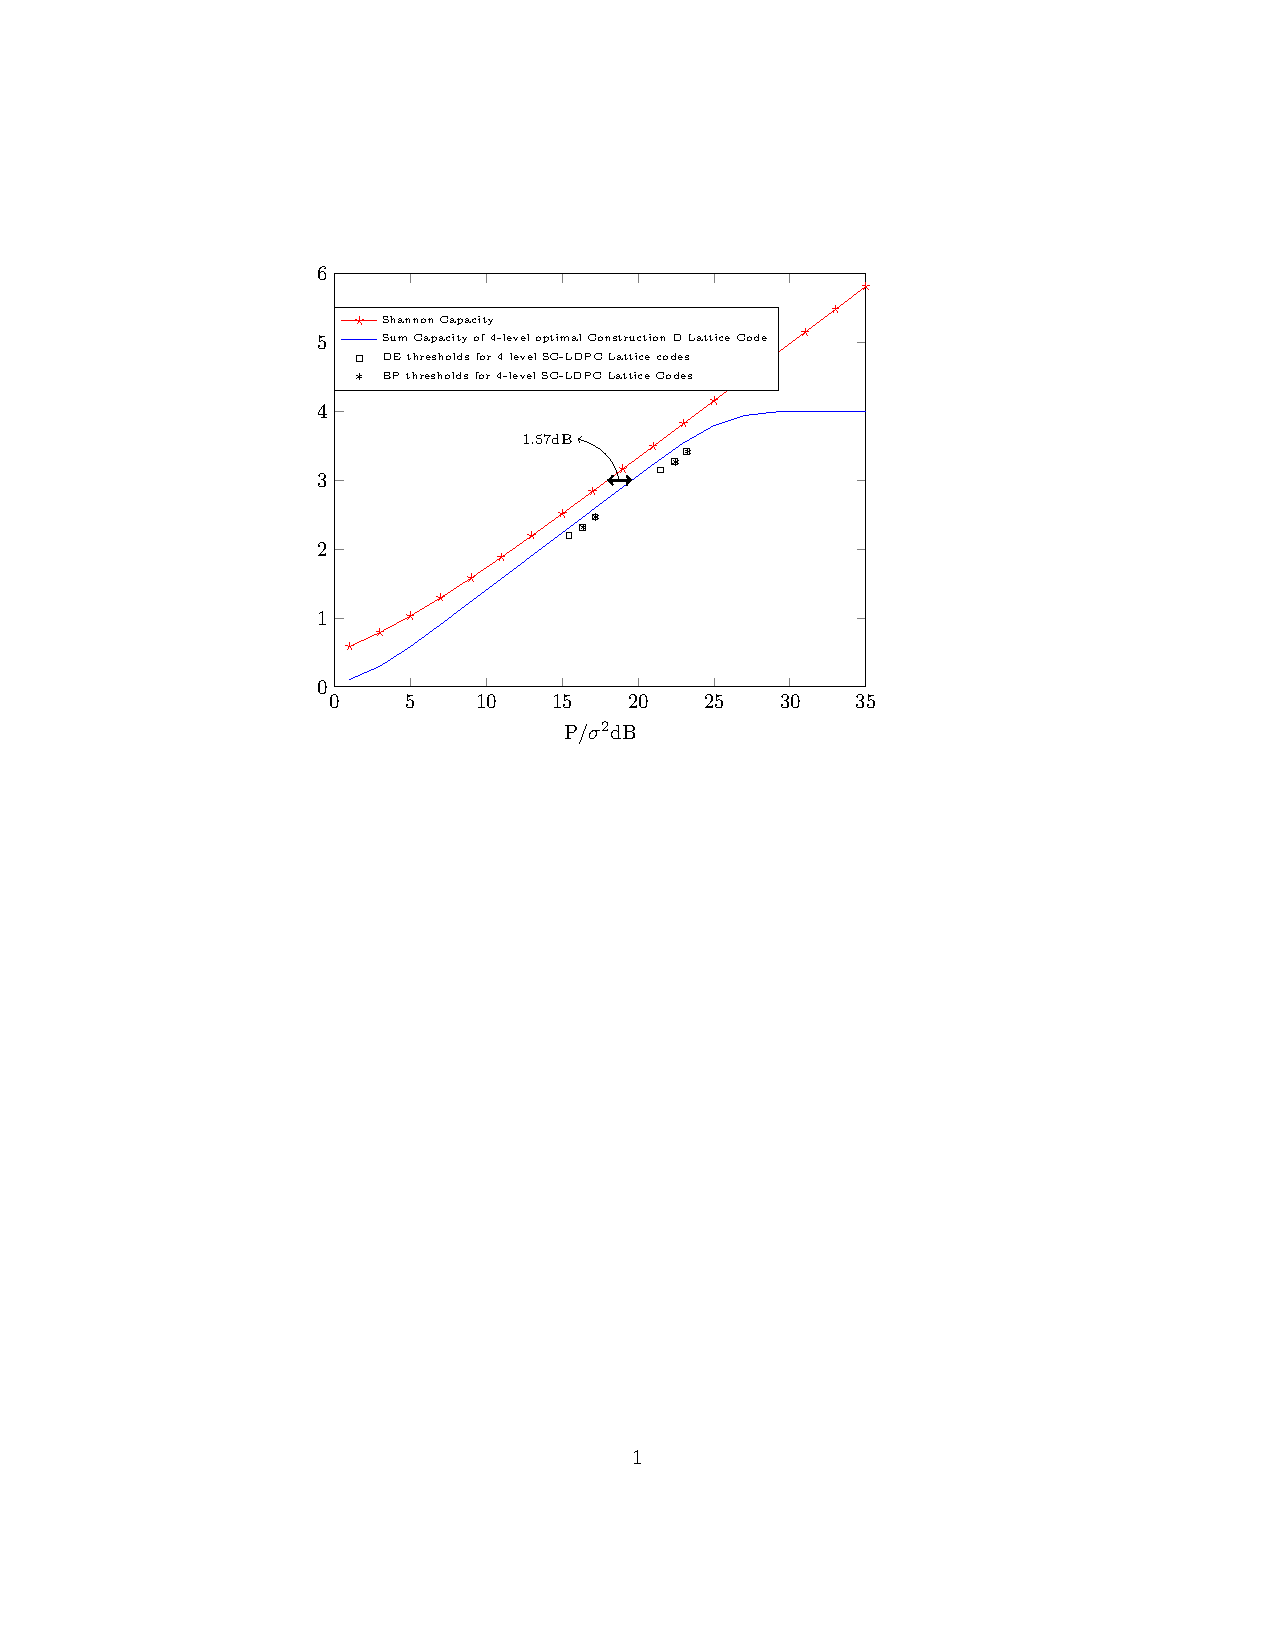
\includegraphics[width=3.5in]{ShapingLoss_Final_CTW}
        \end{center}
    \end{figure}
\end{frame}

\begin{frame}\frametitle{Concluding Remarks}
    \begin{itemize}
        \item Multilevel constructions - efficient ways to decode integer combinations
               \vspace{5pt}
        \item Need capacity achieving nested codes
                \vspace{5pt}
        \item Multilevel construction is provably good under message passing decoding
               \vspace{5pt}
               \pause
        \item \red{Coding schemes based on Binary LDPC codes and iterative decoding suffice}
    \end{itemize}
\end{frame}

\end{document}